\documentclass[11pt]{amsart}
\usepackage{geometry}                % See geometry.pdf to learn the layout options. There are lots.
\geometry{letterpaper}                   % ... or a4paper or a5paper or ... 
%\geometry{landscape}                % Activate for for rotated page geometry
%\usepackage[parfill]{parskip}    % Activate to begin paragraphs with an empty line rather than an indent
\usepackage{graphicx}
\usepackage{amssymb}
\usepackage{epstopdf}
\usepackage{hyperref}
\usepackage{graphicx}
\usepackage{subfigure}


\theoremstyle{mydef}
\newtheorem{definition}{Definition}
\newtheorem{conj}{Conjecture}[section]
\newtheorem{thm}{Theorem}[section]



\DeclareGraphicsRule{.tif}{png}{.png}{`convert #1 `dirname #1`/`basename #1 .tif`.png}

\title{On (mod n) Spirals}
\author{Andrew Reiter\\
arr@watson.org}
\author{Robin Young\\
young@math.umass.edu}
%\date{}                                           % Activate to display a given date or no date

\begin{document}
\maketitle
\section{Introduction}
This note is intended to introduce the process of constructing (mod n) spirals and the idea of a \textit{complete spiral}.  It also introduces a few theorems, with proof, related to patterns seen in the construction of \textit{complete spirals}; regarding the lengths of sides, iteration counts, and ending corners of these objects. Further, from the theorem on iteration counts one sees that these complete spirals provide a (manual) process for discovering the \textit{greatest square divisor} of integers $n \ge 2$. Lastly, grayscale visualizations of a number \textit{complete spirals} were generated to further the investigatory process and are shared herein. While not inspired by Ulam's Spiral \cite{Ulam}, the construction of  a (mod n) spiral is similar in nature. The author's are unaware of other work or literature on this topic, so have no references other the couple related to code; in part this is why the note has been written. Further, the investigation provided some bit of fun which has made it worthwhile.

\section{Spiral Construction}
Here describes the construction of a (mod n) spiral and much of the notation defined and assumptions made here are used with same notion after this section.

Let $n \in \mathbb{Z}$ and $n \ge 2$ and so $\mathbb{Z}/n\mathbb{Z} = \{ 0, 1, ..., n-1 \}$. Let $L$ be a square lattice. 

Choose a point $l_0 \in L$ and it will be the starting point of the spiral; choose $l_0 = (0, 0)$, the origin. Let $l^*_0$ be the value assigned to the point $l_0$. We want to assign the first element of $\mathbb{Z}/n\mathbb{Z}$ to the first point in the spiral, thus, we assign $l^*_0 = 0$. Now, we wish to choose a second point in the spiral, $l_1$, by moving in the positive $x$ direction by one unit and assign it the second value of $\mathbb{Z}/n\mathbb{Z}$. So we have $l_1 = (1, 0)$ and $l^*_1 = 1$.  We will continue to choose points $l_i$ and assigning values from $\mathbb{Z}/n\mathbb{Z}$ in an increasing order.

\begin{figure}[h]
\centering
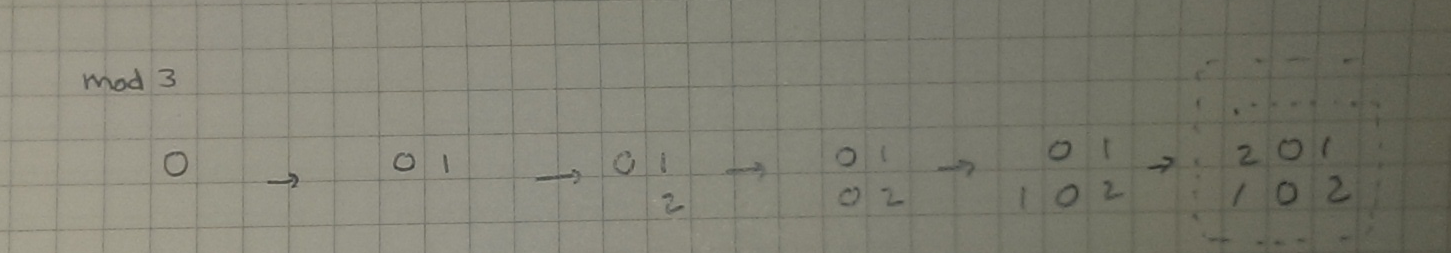
\includegraphics[scale=0.3]{mod3basic.png}
\caption{Building a (mod 3) spiral}
\label{fig:mod3spiral}
\end{figure}

To continue this process, let us try to visualize us being on the lattice work itself. Orient your mind so that previous move to $l_1$ was you ``moving forward''. With current position $l_1$, check the lattice point to your right: if it is assigned a value already, move ``forward'' to the next lattice point. However, if the lattice point to the right was \emph{not} occupied, then you ``turn right'' and ``move forward'' to occupy it. You are now at $l_2$ and have $l^*_2 = 2$ and, based on above, $l_2 = (1, -1)$. . You repeat this pattern of ``looking right'' to determine if you should ``turn right'' or keep ``moving forward'' and then assigning values from $\mathbb{Z}/n\mathbb{Z}$. Continuing on with the lattice points we find $\{ l_i \}^{6}_{i=3} = \{  (0, -1), (-1, -1), (-1, 0), (-1, 1) \}$

At some point, the process will reach a lattice point $l_i$ in which $l^*_{i-1} = n-1$. This is means an \textit{iteration of (mod n)} has occurred and we assign $l^*_i = 0$. This restarts going through values of $\mathbb{Z}/n\mathbb{Z}$. The (mod n) spiral is the set of tuples $\{ (l_0, l^*_0), (l_1, l^*_1), ... \}$ 





\begin{figure}[h]
\centering
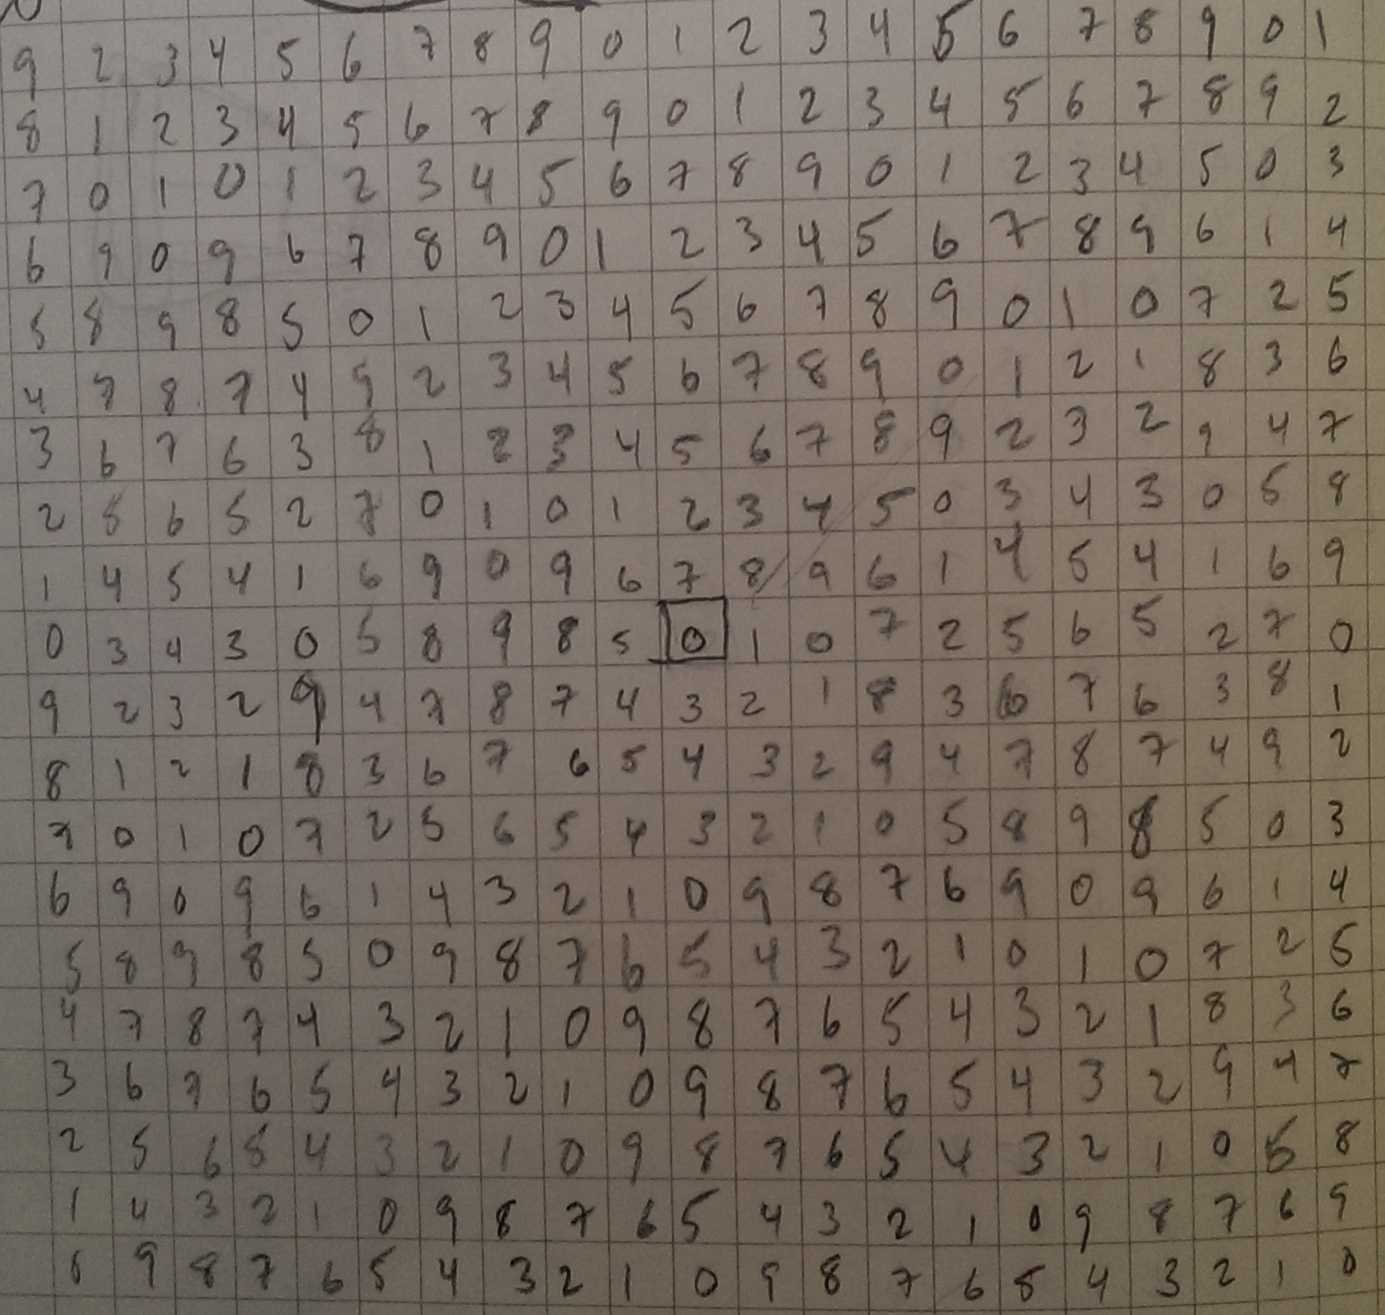
\includegraphics[scale=0.3]{mod10.png}
\caption{a (mod 10) spiral with starting 0 enblocked}
\label{fig:mod10}
\end{figure}

The purpose of inventing notation for the lattice points is to help give a scalar mapping into the lattice based on the spiral. Currently it is not used, but could be used in research investigating patterns on the diagonals of generated spirals. In looking at the construction of a spiral based on $\mathbb{Z}/10\mathbb{Z}$ in figure \ref{fig:mod10}, with the starting point $l_0$ with value $l^*_0 = 0$ marked by a box, one can begin to see the diagonal patterns one might wish to investigate.




\section{complete spiral}
The initial interest in generating spirals of increasing size for various $\mathbb{Z}/n\mathbb{Z}$ was se more of the diagonal patterns as referred to above and seen in figure \ref{fig:mod10}. In thinking about how to do this in strict manner, the following definitions were created after some thought:

\begin{definition}[complete spiral]
A complete spiral is achieved when in the spiral construction you reach a point where $l^*_i = n-1$, $l_i$ is on a corner, and the lengths of the outermost sides are equal.
\end{definition}

\begin{definition}[$k^{th}$ complete spiral of $\mathbb{Z}/n\mathbb{Z}$]
The first complete spiral reached in the spiraling process is k=1, or $1^{st}$ complete spiral,  $Ond^1_n$. Spiraling further and reaching other complete spirals, we increment $k$ and have $Ond^k_n$.
\end{definition}

The word \textit{Ond} is ``spiral'' in Swahili.

\begin{definition}[Iterations of  $\mathbb{Z}/n\mathbb{Z}$ in $Ond^k_n$]
The number of times $\mathbb{Z}/n\mathbb{Z}$ is used in order to reach the $k^{th}$ square is the iteration count.
\end{definition}

\begin{figure}[h]
\centering
\subfigure{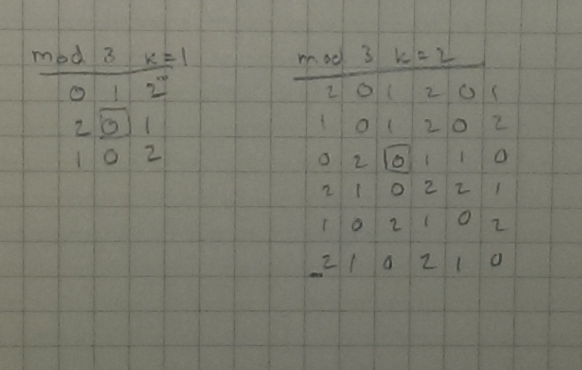
\includegraphics[height=4cm]{mod3k12.png}}
\subfigure{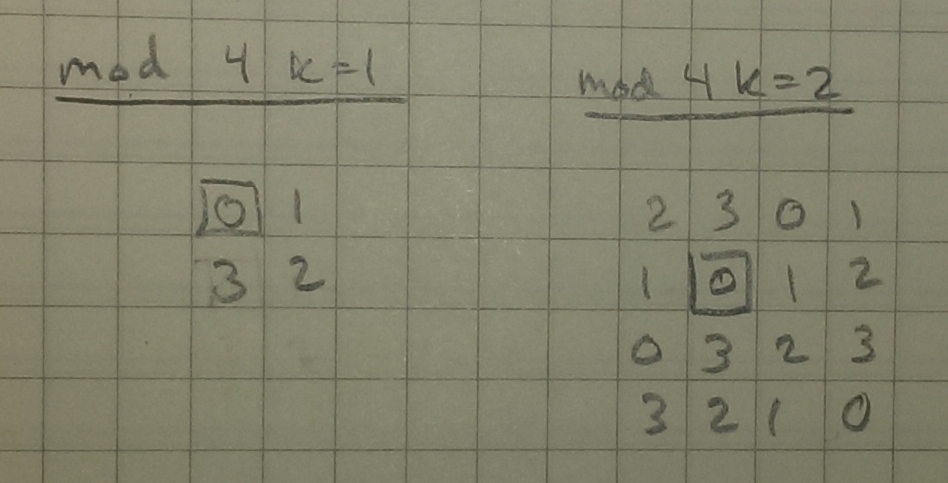
\includegraphics[height=4cm]{mod4.png}}
\caption{$Ond^1_3$ and $Ond^2_3$ on the left, $Ond^1_4$ and $Ond^2_4$ on the right}
\label{fig:mod34}
\end{figure}

We see in figure \ref{fig:mod34} the cases of (mod 3) for $k=1,2$.  In the case of $Ond^1_3$, it is a 3-by-3 square and took 3 iterations of $S_3$. For $Ond^2_3$, it results in 6-by-6 and 12 iterations. With $Ond^1_4$, we see 2 and 1, and $Ond^2_4$, we see 4 and 4.

The author pursued generating spirals with pencil and paper in a methodical manner to  create sets of complete spirals for various values of $n$ and $k$. While tedious and not exactly related to the initial goal of looking at diagonal patterns, it helped to realize there seemed to be patterns found in the construction of the spirals. Specifically in the sizes of the complete spirals, iteration counts, and where the last lattice point rested; this led the author to investigate what the patterns were.

\subsection{On the side lengths and iterate counts of $Ond^k_n$}
In order to investigate these patterns, the author determined that more data was needed and, due to the tedium of pencil and paper, a program should be written to generate complete spirals \cite{PySquare}. This allowed the author to generate a larger number of complete spirals and collect data on lengths, iterations, and ending points. 

In looking at the initial data, for small choices of $n, k$, a few patterns in tuples of (lengths, iterations) were found, including $(kn, k^2 n)$, $(\frac{kn}{2}, \frac{k^2 n}{4})$, and $(\sqrt{n}k, k^2)$. Not proving suitable, the prime factorization of $n$ for each complete spiral $Ond^k_n$ with the lengths and iteration data was generated for analysis. From this data, the author determined there was a relation involved with finding the greatest square divisor of $n$, which led to the following theorems.

\begin{thm}[Length of Sides of $Ond^k_n$]
Let $\lambda$ be the length of the sides of $Ond^k_n$. If $s$ is the greatest square divisor of $n$, then $\lambda = \frac{kn}{\sqrt{s}}$.
\label{lenthm}
\end{thm}

\begin{proof}
Fix an integer $n \ge 2$.  Let $\lambda$ be the length of the side of a complete spiral. In order to achieve some $Ond_n$ for side length $\lambda$, then it must be that $n \vert \lambda^2$. Realize that we can write $n = q^2_1 q_2$ where $q_2$ is square-free. In the case of $n$ being square free, $q^2_1 = 1$ and $q_2 = n$. Then we must have $\lambda = k q_1 q_2$ and that each $k = 1, 2, 3...$ satisfies this. Thus, $Ond^k_n$ has side $\lambda = k q_1 q_2$. Since, $n = q^2_1 q_2$, then we have $\lambda = \frac{kn}{q_1}$ and we see $\sqrt{s} = q_1$ since $q^2_1$ is the greatest square divisor of $n$.
\end{proof}

\begin{thm}[Iteration Count of $Ond^k_n$]
Let $\xi$ be the iteration count  of $Ond^k_n$. If $s$ is the greatest square divisor of $n$,  then, $\xi = \frac{k^2n}{s}$.
\end{thm}


\begin{proof}
This follows from the proof of theorem \ref{lenthm}. Realize that $\xi n = \lambda^2 = \frac{k^2}{s}$ and so $s = q^2_1$. Thus $s$ is the greatest square divisor of $n$.
\end{proof}



One will note that in the case where $n$ is a product of just one of each prime factor, these reduce to $\lambda = k n$ and $\xi = k^2 n$. These can also be considered an upper bound for all cases. Further, it should be noted that if $n$ is square free, then the upper bound is achieved. One might consider these to be the least robust in the case of length and iteration counts.

\subsubsection{Construction to Find G.S.D.}
A most interesting aspect to this process of complete spiral construction is the connection to greatest square divisor of some integer $n$. To see this more clearly, choose some $n$ and construct, by hand, the $Ond^1_n$. At this point, you know $\lambda$ and $\xi$, so pick one, substitute $k = 1$ and solve for $s$. So from a constructivist approach we find the greatest square divisor.

\subsection{Ending Corner of $Ond^k_n$}

Another pattern in the generation of \textit{complete spirals} that was noticed is related to which corner the last lattice point comes to rest. It seems to end on either the top right or bottom left corner and this depends on values of $n$ and $k$. One can see this in figure \ref{fig:mod34}. 

\begin{thm}[Ending Corner]
If $l_{max} \in L$ is the last lattice point in the complete spiral $Ond^k_n$, then $l_{max}$ is either the top-right corner or bottom-left corner. If $N$ even, then $l_{max}$ will always be the bottom-left corner. If $n$ odd and $k$ odd, then $l_{max}$ will be the top-right corner of $Ond^k_n$. If $N$ odd and $k$ even, then $l_{max}$ will be the bottom-left corner.
\end{thm}

It is worth noting that $l_{max} = l_{\xi(n, k)\vert \mathbb{Z}/n\mathbb{Z} \vert - 1}$, due to starting with $l_0$.

\begin{proof}
Writing the spiral for $\mathbb{N}$, make a 1-to-1 mapping from $\mathbb{Z}/n\mathbb{Z}$ map to a subset of it. Endings end on perfect squares. Perfect squares are on diagonals of upper right and lower left. Evens are on the lower left. Perfect square of evens is even, and Perfect square of  odds are odd. So, in iterating onward, one set, we have all evens, so maps to lower left. other case, we swap between odd/even and thus map upper right/lower left alternating.
\end{proof}

\subsection{Cases Verified}
I have verified the conjectures on length, iteration count, and end corners for $n=2\ldots450$ and $k=1\ldots5$. This code may be found at \cite{PySquare}. At this location, if you view the file \textit{run.log} you will see log output of the code running.

\subsection{Grayscale Visualization}

In the process of investigating sizes and iteration counts of $Ond^k_n$, I implemented a method to map the generated spirals to grayscale images. This works best for positive integers, $n$, less than 256. I define the map as $f : \{ 0, 1, \ldots, n-1 \} \mapsto \{ 0, floor(\frac{255}{n}), 2floor(\frac{255}{n}), \ldots, (n-1)floor(\frac{255}{n}) \}$. The mapping $f$ takes $\mathbb{Z}/n\mathbb{Z}$ to a set of brightness values. These brightness values are easily used to create grayscale images.

An example of this is $Ond^{29}_{28}$ seen in figure \ref{fig:viz2928} and $Ond^{30}_{16}$ seen in figure \ref{fig:viz1630}.

\begin{figure}[h]
\centering
\includegraphics[scale=0.7]{N28k29a.png}
\caption{grayscale visualization of $Ond^{29}_{28}$}
\label{fig:viz2928}
\end{figure}

\begin{figure}
\centering
\includegraphics[scale=1]{spN16k30.png}
\caption{grayscale visualization of $Ond^{30}_{16}$}
\label{fig:viz1630}
\end{figure}

However, due to computation time taking to generate the spirals and the images, I only generated $N=2...30$ for $k=1...50$. They may be viewed at \cite{GraySquare}.

\section{Conclusion}
This note has introduced (mod n) spiral construction and the idea of \textit{complete spirals} with respect to (mod n) spirals. This note also gives 3 theorems with proof about some features of these spirals. Also introduced is a grayscale visualization of these spirals. 

\subsection{Future Work}
The diagonal patterns in the larger $k$ $Ond^k_n$ spirals would make for interesting to see how to categorize and determine their generators. In a private conversation \cite{Kusner} suggested also looking at the angular velocity of spiral growth, which might be fun.

It would be of interest to think about looking at how spiraling might work for cubes or higher dimensional squares, since the lattice is the basis for the spiral. Further, it might be interesting to see how one might spiral with objects in $\mathbb{R}^2$ such as a triangle.

\subsection{Acknowledgments}
Recognizing Veracode Inc for providing time to think about this and Jared Carlson of Veracode for some initial discussion.

\begin{thebibliography}{1}
\bibitem{Ulam} Wolfram Mathworld, ``Prime Spirals'', \url{http://mathworld.wolfram.com/PrimeSpiral.html}
\bibitem{PySquare} A. Reiter, \url{https://github.com/cwcomplex/modNspirals}
\bibitem{GraySquare} A. Reiter, \url{https://github.com/cwcomplex/modNspirals/tree/master/somegrey}
\bibitem{sqmaxes} A. Reiter, \url{https://github.com/cwcomplex/modNspirals/blob/master/squareoff.py}
\bibitem{Kusner} R. Kusner, A. Reiter, \textit{private email correspondence}

\end{thebibliography}



\end{document}  